\section{Het digitale filter}

Met het MATLAB bestand voor een 1dB Chebychev filter hebben we een code geschreven voor het filter. 
Op het begin van de code worden alle waardes berekend in defines.
Deze waardes worden vervolgens gebruikt in de ISR van de ADC. De code is gebaseerd op de tekening in MATLAB.

\begin{figure}[!h]
    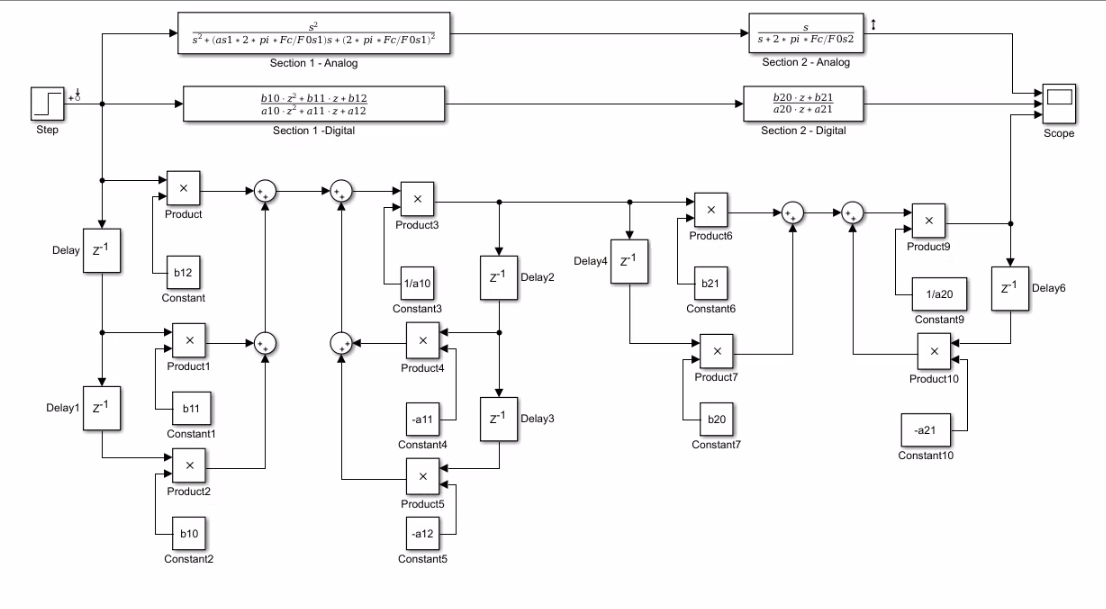
\includegraphics[width=0.9\linewidth]{matlab/MATLAB tekening.png}
	\caption{Tekening in MATLAB}
	\label{fig:matlabDrawing}
\end{figure}

Het digitale filter is op dit moment niet functioneel. 
